% !TeX root = ../mat_mod2.tex

\section{
  Итерационный режим с комбинированием оптимизирующих вставок разной <<длины>>
}
\label{sect:5.3}
\setcounter{equation}{0}

Начиная с настоящего раздела мы рассматриваем конструкции решения задачи
(\ref{4.4.13}) с использованием оптимизирующих вставок. Основное внимание
здесь и далее уделяется итерационным алгоритмам на основе подходов,
сформулированных в заключении предыдущей главы. Будем придерживаться
обозначений раздела~4.4 в части описания элементов <<большой>> задачи
(см. (\ref{4.4.13})), а, в части описания локальных задач, --- обозначений
раздела~4.3. Итак, схема ДП раздела~4.3 используется при построении
оптимизирующих вставок, направленных на обеспечение   локального улучшения
ДР <<большой>> задачи. Последняя рассматривалась на уровне построения
алгоритмов и программ в реализации, ориентированной на применение для
целей маршрутизации движения инструмента при листовой резке на станках
с ЧПУ.

Сначала совсем кратко напомним итерационную процедуру, в рамках которой
предполагалось сочетание оптимизирующих вставок разной <<длины>>. Как и
в разделе~4.4, полагаем, что $\nn\in \bbn$ определяет количество мегаполисов
<<большой>> задачи; значение $\nn$ полагается достаточно большим, а потому
непосредственное применение ДП (см. раздел~4.3) для целей <<глобальной>>
оптимизации практически невозможно. Пусть, однако, задано число
$N\in \bbn,$ определяющее размер или <<длину>> вставки; при этом
в последующих конструкциях полагается, что при данном значении $N$ в
локальной задаче маршрутизации, возникающей при построении вставки,
процедура на основе ДП уже позволяет осуществить вычисления, приводящие
к построению оптимального локального решения (имеется в виду вариант
задачи (\ref{4.3.3})) и нахождению значения (\ref{4.3.5}), то есть
экстремума локальной задачи.

Некоторую проблему составляет выбор начала вставки, которое в разделе~4.4
было обозначено через $\nu$ (см. (\ref{4.4.24})). Конечно, данный параметр
можно выбрать как угодно, соблюдая (\ref{4.4.24}); при этом, как показано в
главе~4, значение критерия <<большой>> задачи не ухудшится. Однако желательно
устраивать вставку там, где она обеспечит реальное улучшение совокупного
критерия; таким образом, <<момент>> начала вставки надо искать, исходя из
соображений, связанных с улучшением критерия. В конце главы~4 были намечены
некоторые подходы к выбору параметра $\nu.$ Все эти подходы связывались с
организацией той или иной итерационной процедуры. Мы начнем сейчас с
рассмотрения того варианта данной процедуры, когда для поиска $\nu$
привлекается система вставок меньшего размера. Последнее существенно, так
как на каждом этапе основной итерационной процедуры  приходится (в рамках
данного подхода) проигрывать реализацию поисковых вставок многократно.
Цель этих построений, как  уже отмечалось в главе~4, состоит в определении
такого значения $\nu,$ для которого исходное эвристическое ДР было бы
наиболее <<податливо>> к улучшению. Последнее же предлагается осуществлять
с помощью вставки большего размера (большей <<длины>>). Итак, мы рассматриваем
вставки разной <<длины>>, придавая значению $N$ одно из двух значений
$$(N = N_1) \vee (N=N_2),
$$
где $2 \leqslant N_1 < N_2 <\nn.$ Соответственно у нас на каждом этапе
возникают (зондирующие) $N_1$-вставки и одна рабочая $N_2$-вставка.

При этом, как уже отмечалось в заключительной части главы~4, значение
$N_1$ подбирается таким, чтобы было возможно <<прорешать>> все локальные
маршрутные задачи в диапазоне $\ov{0,\nn-N_2}.$ Правда при решении упомянутых
локальных задач не требуется находить оптимальные маршрут и трассу; требуется
только <<быстро>> определять экстремумы; в настоящем варианте для этого
использовалось ДП в духе процедуры (\ref{4.3.13}), финалом которой является
определение экстремума локальной маршрутной задачи.

%*******************************************************************************
В примере рассматривался случай $\mathbf{n}=75$ и $|\mathbf{K}|=37$. Размеры вставок
были выбраны следующими: $N_1=12$, $N_2=24$.
Функции стоимости выбраны такими же, как в предыдущем примере (из раздела
5.2). Количество итераций равнялось
15. Начальный вариант посчитан с использованием эвристического итерационного
алгоритма, значение полученного критерия равно 250,79. Результат, достигнутый
после применения вставок ДП равен 249,3. Общее время счета составляет 17
мин. 3 сек. Маршрут и трасса показаны на рис. \ref{DP_Inserts_Result}.

\begin{figure}
  \begin{center}
  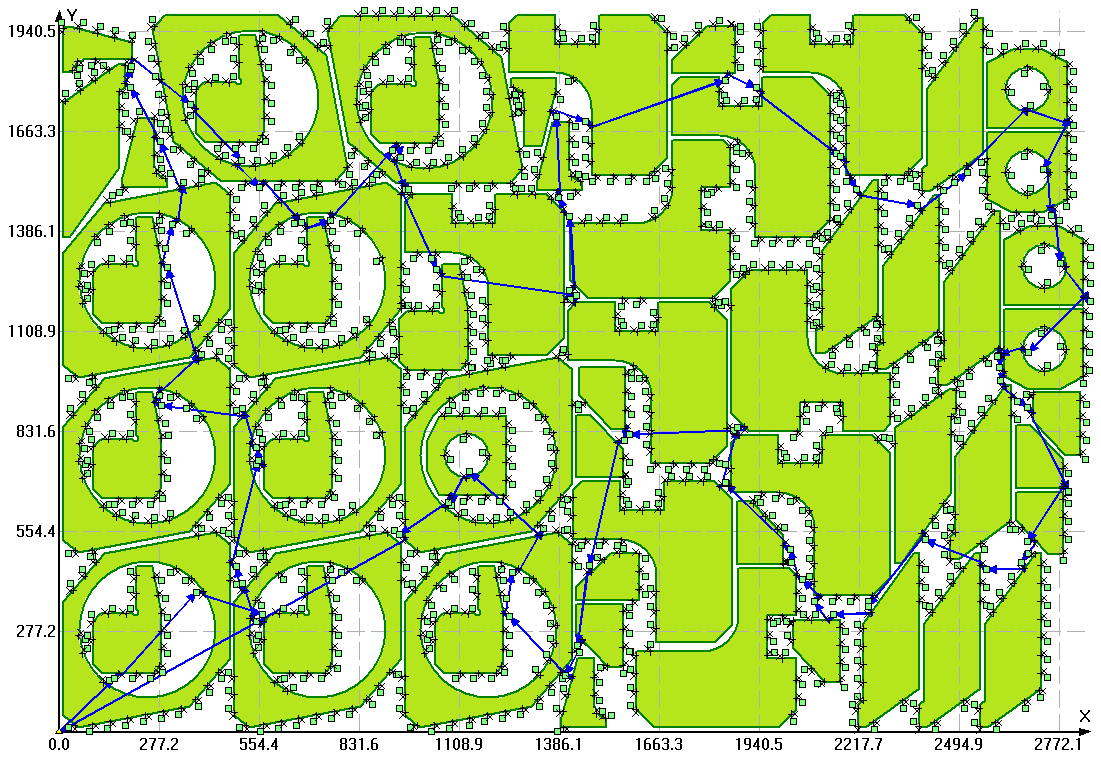
\includegraphics[width=0.9\textwidth]{routing_75_checking_ins.png}
  \caption{
    Траектория, полученная с использованием эвристического алгоритма
    с~улучшающими вставками ДП
    }
  \label{DP_Inserts_Result}
  \end{center}
\end{figure}
